%!TEX root = ../docu.tex
\section{Konzept}
\subsection{Grundkonzept}

Im folgenden wird die Konzeptionierung der Anwendung beschrieben ,welche im spteren implementiert wird. heirbei handelt es sich um eine applikation hauptsächlich für das abspielen von Hörbüchern im audioformat MP3. Die applikation soll so einfahc wie möglich gestaltet und zweckgerichtet sein.

die applikation soll dem benutzer ermöglichen hörbücher abzuspielen, welche er vorher auf sein mobiles endgerät abgelegt hat. hierfür muss die applikation einen einstellungsmöglichkeit beinhalten.

über diese einstlelungen muss dem benutzer möglichsein de speicherort frei wählen zu können. über diese einstellungsparameter ist es der anwendung nun möglich alle audiodateien aufzulisten und abspielne zu können.

die auflsitung filtert alle nciht abspielbaren daten und ermöglicht desweitern in unterodernen zu navigieren. ein element der lsite stellt dabei entweder eine audidatei doer ein utneroderner dar. 

\begin{figure}
\begin{center}
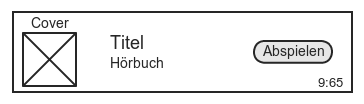
\includegraphics[scale=0.8]{images/listitem}
\caption{Mockup für ein Listenelement}
\label{mocklistel}
\end{center}
\end{figure}

die abnildung \ref{mocklistel} beschreibt ein soclhes element. ein elemnt enthält das cover des hörbuches sowie der titel und die genau abspielzeit. über ein weiteres element soll es möglichsein eine aktion auszuführen welche das abspielen der jeweiligen audiodatei ermöglicht.

aus dieser auflistung herraus soll es möglich sein audiodateien abspielen zu können. deshalb muss eine schnittstelle zur üebrtragung der informationen zur player komponente erfolgen.

diese komponente ist für das abspielne zuständig. sie empfängt emfängt die anweisung zum abspielen der audiodatei und spiel dieses datei ab.

\begin{figure}
\begin{center}
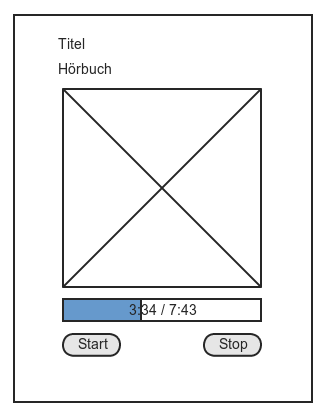
\includegraphics[scale=0.6]{images/playerkomp}
\caption{Schematische Darstellung der Abspiel-Komponente}
\label{playerkomp}
\end{center}
\end{figure}

die palyer komponente in abbildung \ref{playerkomp} dargestellt soll es ermöglichen das abspielen zu steuern. dies beinhaltet das stopen pausieren und andere funktionen. desweitern soll erkennarseinw elche audiodatei abgespielt wird. eine vorschritsanzeige lässt erkennen wie viel von der audio datei bisher abgespielt wird sowie die gesamtlänge der audiodatei.

\begin{figure}
\begin{center}
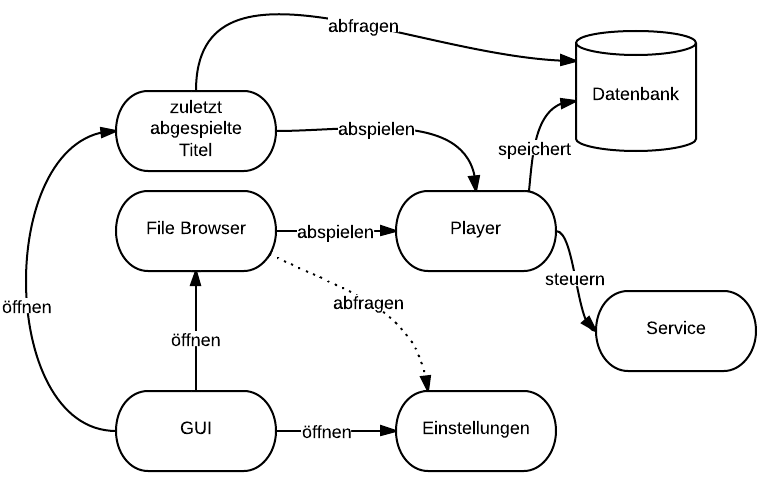
\includegraphics[scale=0.6]{images/konzept}
\caption{Schematische Darstellung der Anwendung}
\label{konzept}
\end{center}
\end{figure}

wird die anwendung geschlossen soll die wiederdabe nciht abbrechen der nutzer soll immernoch in der lage sein die abgespielte audiodatei zu hören.

die anwendung soll in der alge sein abbrüche der wiedergabe zue rknnen und diese punkte zu speicher. der benutzer soll aus diesen informationen eine möglichkeit haben, an diesen punkten die wiedergabe vorzusetzen.

die eingabe erfolgt durch ein übliches touchscren display und soltle dahingehen obtimiert sein. hierzu gehört klare und einfache programmstrukturen sowie ausreichend droße fläschen für bedienelemente und steuerung von programmfunktionen.

die gesammte progrmamstruktur muss os aufgebaut sein um eine weiteretwicklung und implementierung neuer funrktionen zu ermöglichen.
